\documentclass{beamer}

\usepackage[utf8]{inputenc}
\defbeamertemplate{description item}{align left}{\insertdescriptionitem\hfill}

\usepackage{hyperref}
\hypersetup{
    colorlinks=true,
    linkcolor=blue,
    filecolor=magenta,      
    urlcolor=cyan,
}



%Information to be included in the title page:
\title{How did the acceptance of Social Distancing evolve during the Covid-19 pandemic in New York City?}
\subtitle{Exam project for Management of Scientific Data}
\author{Anna Sterzik}
\institute{Friedrich Schiller Universität Jena}
\date{\today}



\begin{document}

\frame{\titlepage}
\begin{frame}
\frametitle{Table of Contents}
\tableofcontents
\end{frame}

\section{Data Management Plan}
\begin{frame}
\frametitle{Project Information}
\setbeamertemplate{description item}[default]
\begin{description}[style=multiline]
\item[Project name:] How did the acceptance of Social Distancing\\ evolve during the Covid-19 pandemic in New York City?
\vfill
\item[Creator:] Anna Sterzik
\vfill
\item[Affiliation:] Friedrich Schiller University Jena
\vfill
\item[Template:] DCC Template
%Project abstract:
%The 311 Service Requests in New York City will be used to investigate how the acceptance of Social Distancing
%measures evolved during the Covid-19 pandemic in New York City. Therefore violations of Social Distancing rules
%will be analysed over time.
Last modified: 10-08-2020
\item The tool \href{https://dmponline.dcc.ac.uk/}{DMPonline} was used
\end{description}

\end{frame}
\begin{frame}
\frametitle{Preexisting Data}
\begin{itemize}
\item Pre-existing data from \href{https://data.cityofnewyork.us/Social-Services/311-Service-Requests-from-2010-to-Present/erm2-nwe9}{311 Service Requests from 2010 to Present}.
\vfill
\item Initial Data Filtering:
\setbeamertemplate{description item}[align left]
\begin{description}[style = multiline]
\item [Dates:] 020/03/01 - 2020/08/11
\item [Description:] Including "Social Distancing"
\end{description}
\vfill
\item raw data volume: 12.7 GB
\vfill
\item Data Format: saved as .csv
\vfill
\item Licence: Open Data Law(?)
\vfill
\item Accessed/Downloaded 2020/08/10 22:14:39 CEST
\end{itemize}
\end{frame}
\begin{frame}
\frametitle{Generated Data}
\begin{itemize}


\item Data will be filtered, analyzed and visualized using jupyter notebooks, such that there is no need to modify the raw data. Everything will be done
by the skripts.
\vfill
\item Required additional storage space for processed data and secondary outputs therefore negligible.
\vfill
\item Formats: ipynb and pdf and tex
\vfill
\item Versioning will be done with git.
\end{itemize}
\end{frame}

\begin{frame}
\frametitle{Documentation and Metadata}
\begin{itemize}
\item Software versions used for this project:
\vfill
\item Documentation will be provided as a README
\vfill
\item Provenance will be handled by \href{https://github.com/Sheeba-Samuel/ProvBook}{ProvBook}
\end{itemize}
\end{frame}
\begin{frame}
\frametitle{Not applicable}
\begin{itemize}
\item Ethics and Legal Compliance
\end{itemize}
\end{frame}
\begin{frame}
\frametitle{Storage and Backup}
\begin{itemize}
\item Data will be stored with URZ, on github and on a DVD/USB stick (3-2-1 Backup rule)
I will be responsible for backing up onto USB stick, URZ and github are managed(?)
\vfill
\item Data will be freely available for everyone at all times via github. (Therefore no security concerns)
\end{itemize}
\end{frame}
\begin{frame}
\frametitle{Selection and Preservation}
\begin{itemize}
\item Critical part of this project is the created software only, not the third party data which is already taken care of by 311 Service Calls data base. Therefore this needs
to be preserved
\vfill
\item The data will be preserved in a github repository,usb and urz.
\end{itemize}
\end{frame}
\begin{frame}
\frametitle{Data Sharing}
\begin{itemize}
\item How will you share the data?
github weil es software project ist.
\vfill
\item Are any restrictions on data sharing required?
No restrictions required.
\end{itemize}
\end{frame}
\begin{frame}
\frametitle{Responsibilities and Resources}
\begin{itemize}
\item Who will be responsible for data management?
I will be responsible for all that stuff because it is only a very small project.
\vfill
\item What resources will you require to deliver your plan?
Only ressources required is storage capacity from URZ.
\end{itemize}
\end{frame}
\section{Description of the Dataset}
\begin{frame}
\frametitle{311 Service Requests in New York City from 2010 to present}
\begin{itemize}
\item Non-emergency Social Service Requestss
\item Provider: DoITT Department of Information Technology \& Telecommunications
\item Owner: NYC OpenData
\item 41 Columns in the Dataset include Unique Key, Information about Dates (Opening, closing), Agency, Complaint Type, Location Information
\item Each row is a service request
\end{itemize}
\end{frame}
\section{Quality Control}
\begin{frame}
\frametitle{Quality Control}

\begin{itemize}
\item Quality control will be done using \href{https://openrefine.org/}{OpenRefine}
\vfill
\item The database states:\\
``NOTE: This data does not present a full picture of 311 calls or service requests, in part because of operational and system complexities associated with remote call taking necessitated by the unprecedented volume 311 is handling during the Covid-19 crisis. The City is working to address this issue.''
\vfill
\item One can also see at first glance that there are several missing values
\end{itemize}
\end{frame}
\begin{frame}

\frametitle{Facets}
\begin{columns}
\column{0.5\textwidth}
\begin{itemize}

\item Facets can be used to get a better overview over the data in specific columns.
\vfill
\item The Complaint Types and Agency Names seem to be reasonible.

\end{itemize}
\column{0.5\textwidth}
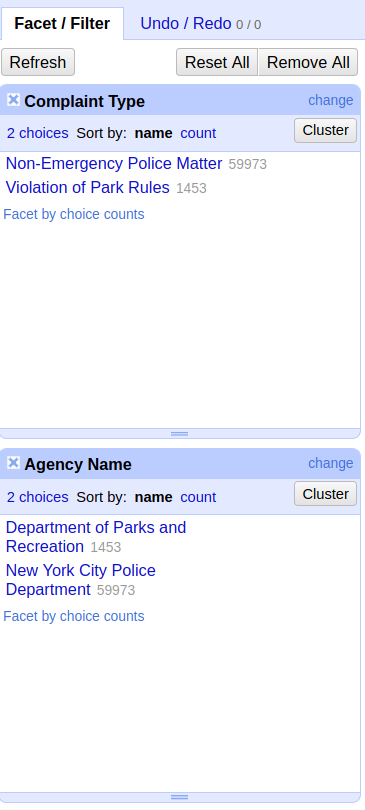
\includegraphics[width = 0.8\textwidth]{pictures/facets.png}
\end{columns}
\end{frame}
\begin{frame}
\frametitle{Clustering}
Clustering is another option to identify erronous data, especially spelling mistakes.
\vfill
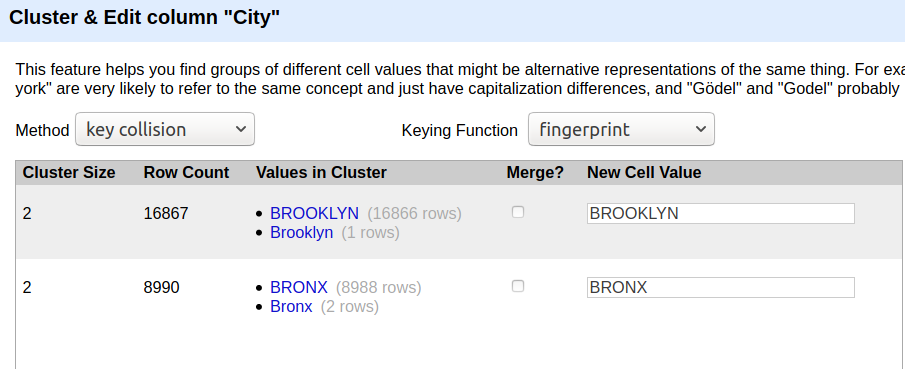
\includegraphics[width = \textwidth]{pictures/clustering.png}
\end{frame}
\begin{frame}
\frametitle{Sorting}
Using OpenRefine one can also sort the values by certain columns. That way one can e.g. determine if the given longitudes and latitudes are reasonable.
Here the latitudes and longitudes seem to be valid for NYC.
\vfill
The same can be done for the dates. The creating dates for example start with 03/28/2020 and end with 08/10/2020. This seems to be right as well, because PAUSE started at 03/22/2020 (https://www.governor.ny.gov/news/governor-cuomo-signs-new-york-state-pause-executive-order)
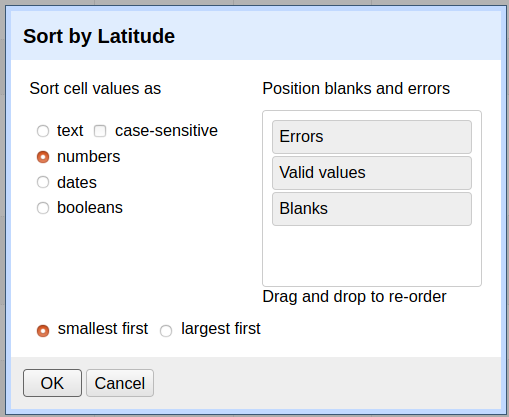
\includegraphics[width=0.5\textwidth]{pictures/sorting.png}
\end{frame}
\begin{frame}
\frametitle{There is more}
Open Refine offers many more tools for Data Cleaning such as:
\begin{itemize}
\item Trimming of Leading and Trailing Whitespaces
\end{itemize}
\end{frame}
\begin{frame}
\frametitle{Saving}
OpenRefine projects can be exported. The resulting files do only contain .txt files and .json files. These files describe all changes made with the data -> provenance is automatically included.
\end{frame}
\section{Data analysis}
\begin{frame}
\frametitle{Data Analysis}
Data analysis will be done using pandas library in a jupyter notebook environment.
\end{frame}
\begin{frame}
\frametitle{Number of Service Calls about 'Social Distancing' in calendar weeks}

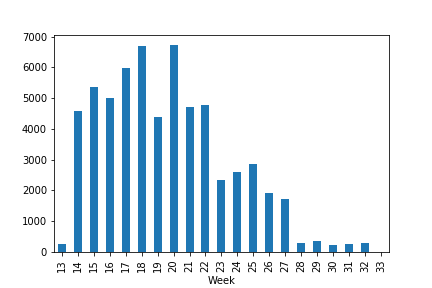
\includegraphics[width=\textwidth]{pictures/bar.png}

\end{frame}
\begin{frame}
\frametitle{Comparison of 'Social Distancing' Service Calls in Bronx and Manhattans}

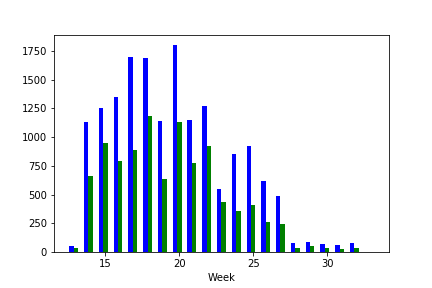
\includegraphics[width=\textwidth]{pictures/comp_bronx_manhattan.png}

\end{frame}
\section{Preservation and Publishing}
\begin{frame}
\begin{itemize}
\frametitle{Preservation and Publishing}
\item Publishing on Github
\vfill
\item Backup copies with the URZ and a USB drive as well
\vfill
\item Material available on Github under a MIT Licence
\end{itemize}
\end{frame}

\end{document}